\documentclass[1p]{elsarticle_modified}
%\bibliographystyle{elsarticle-num}

%\usepackage[colorlinks]{hyperref}
%\usepackage{abbrmath_seonhwa} %\Abb, \Ascr, \Acal ,\Abf, \Afrak
\usepackage{amsfonts}
\usepackage{amssymb}
\usepackage{amsmath}
\usepackage{amsthm}
\usepackage{scalefnt}
\usepackage{amsbsy}
\usepackage{kotex}
\usepackage{caption}
\usepackage{subfig}
\usepackage{color}
\usepackage{graphicx}
\usepackage{xcolor} %% white, black, red, green, blue, cyan, magenta, yellow
\usepackage{float}
\usepackage{setspace}
\usepackage{hyperref}

\usepackage{tikz}
\usetikzlibrary{arrows}

\usepackage{multirow}
\usepackage{array} % fixed length table
\usepackage{hhline}

%%%%%%%%%%%%%%%%%%%%%
\makeatletter
\renewcommand*\env@matrix[1][\arraystretch]{%
	\edef\arraystretch{#1}%
	\hskip -\arraycolsep
	\let\@ifnextchar\new@ifnextchar
	\array{*\c@MaxMatrixCols c}}
\makeatother %https://tex.stackexchange.com/questions/14071/how-can-i-increase-the-line-spacing-in-a-matrix
%%%%%%%%%%%%%%%

\usepackage[normalem]{ulem}

\newcommand{\msout}[1]{\ifmmode\text{\sout{\ensuremath{#1}}}\else\sout{#1}\fi}
%SOURCE: \msout is \stkout macro in https://tex.stackexchange.com/questions/20609/strikeout-in-math-mode

\newcommand{\cancel}[1]{
	\ifmmode
	{\color{red}\msout{#1}}
	\else
	{\color{red}\sout{#1}}
	\fi
}

\newcommand{\add}[1]{
	{\color{blue}\uwave{#1}}
}

\newcommand{\replace}[2]{
	\ifmmode
	{\color{red}\msout{#1}}{\color{blue}\uwave{#2}}
	\else
	{\color{red}\sout{#1}}{\color{blue}\uwave{#2}}
	\fi
}

\newcommand{\Sol}{\mathcal{S}} %segment
\newcommand{\D}{D} %diagram
\newcommand{\A}{\mathcal{A}} %arc


%%%%%%%%%%%%%%%%%%%%%%%%%%%%%5 test

\def\sl{\operatorname{\textup{SL}}(2,\Cbb)}
\def\psl{\operatorname{\textup{PSL}}(2,\Cbb)}
\def\quan{\mkern 1mu \triangleright \mkern 1mu}

\theoremstyle{definition}
\newtheorem{thm}{Theorem}[section]
\newtheorem{prop}[thm]{Proposition}
\newtheorem{lem}[thm]{Lemma}
\newtheorem{ques}[thm]{Question}
\newtheorem{cor}[thm]{Corollary}
\newtheorem{defn}[thm]{Definition}
\newtheorem{exam}[thm]{Example}
\newtheorem{rmk}[thm]{Remark}
\newtheorem{alg}[thm]{Algorithm}

\newcommand{\I}{\sqrt{-1}}
\begin{document}

%\begin{frontmatter}
%
%\title{Boundary parabolic representations of knots up to 8 crossings}
%
%%% Group authors per affiliation:
%\author{Yunhi Cho} 
%\address{Department of Mathematics, University of Seoul, Seoul, Korea}
%\ead{yhcho@uos.ac.kr}
%
%
%\author{Seonhwa Kim} %\fnref{s_kim}}
%\address{Center for Geometry and Physics, Institute for Basic Science, Pohang, 37673, Korea}
%\ead{ryeona17@ibs.re.kr}
%
%\author{Hyuk Kim}
%\address{Department of Mathematical Sciences, Seoul National University, Seoul 08826, Korea}
%\ead{hyukkim@snu.ac.kr}
%
%\author{Seokbeom Yoon}
%\address{Department of Mathematical Sciences, Seoul National University, Seoul, 08826,  Korea}
%\ead{sbyoon15@snu.ac.kr}
%
%\begin{abstract}
%We find all boundary parabolic representation of knots up to 8 crossings.
%
%\end{abstract}
%\begin{keyword}
%    \MSC[2010] 57M25 
%\end{keyword}
%
%\end{frontmatter}

%\linenumbers
%\tableofcontents
%
\newcommand\colored[1]{\textcolor{white}{\rule[-0.35ex]{0.8em}{1.4ex}}\kern-0.8em\color{red} #1}%
%\newcommand\colored[1]{\textcolor{white}{ #1}\kern-2.17ex	\textcolor{white}{ #1}\kern-1.81ex	\textcolor{white}{ #1}\kern-2.15ex\color{red}#1	}

{\Large $\underline{12a_{0115}~(K12a_{0115})}$}

\setlength{\tabcolsep}{10pt}
\renewcommand{\arraystretch}{1.6}
\vspace{1cm}\begin{tabular}{m{100pt}>{\centering\arraybackslash}m{274pt}}
\multirow{5}{120pt}{
	\centering
	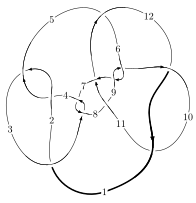
\includegraphics[width=112pt]{../../../GIT/diagram.site/Diagrams/png/916_12a_0115.png}\\
\ \ \ A knot diagram\footnotemark}&
\allowdisplaybreaks
\textbf{Linearized knot diagam} \\
\cline{2-2}
 &
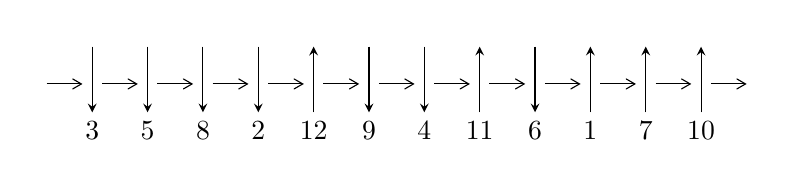
\begin{tikzpicture}[x=20pt, y=17pt]
	% nodes
	\node (C0) at (0, 0) {};
	\node (C1) at (1, 0) {};
	\node (C1U) at (1, +1) {};
	\node (C1D) at (1, -1) {3};

	\node (C2) at (2, 0) {};
	\node (C2U) at (2, +1) {};
	\node (C2D) at (2, -1) {5};

	\node (C3) at (3, 0) {};
	\node (C3U) at (3, +1) {};
	\node (C3D) at (3, -1) {8};

	\node (C4) at (4, 0) {};
	\node (C4U) at (4, +1) {};
	\node (C4D) at (4, -1) {2};

	\node (C5) at (5, 0) {};
	\node (C5U) at (5, +1) {};
	\node (C5D) at (5, -1) {12};

	\node (C6) at (6, 0) {};
	\node (C6U) at (6, +1) {};
	\node (C6D) at (6, -1) {9};

	\node (C7) at (7, 0) {};
	\node (C7U) at (7, +1) {};
	\node (C7D) at (7, -1) {4};

	\node (C8) at (8, 0) {};
	\node (C8U) at (8, +1) {};
	\node (C8D) at (8, -1) {11};

	\node (C9) at (9, 0) {};
	\node (C9U) at (9, +1) {};
	\node (C9D) at (9, -1) {6};

	\node (C10) at (10, 0) {};
	\node (C10U) at (10, +1) {};
	\node (C10D) at (10, -1) {1};

	\node (C11) at (11, 0) {};
	\node (C11U) at (11, +1) {};
	\node (C11D) at (11, -1) {7};

	\node (C12) at (12, 0) {};
	\node (C12U) at (12, +1) {};
	\node (C12D) at (12, -1) {10};
	\node (C13) at (13, 0) {};

	% arrows
	\draw[->,>={angle 60}]
	(C0) edge (C1) (C1) edge (C2) (C2) edge (C3) (C3) edge (C4) (C4) edge (C5) (C5) edge (C6) (C6) edge (C7) (C7) edge (C8) (C8) edge (C9) (C9) edge (C10) (C10) edge (C11) (C11) edge (C12) (C12) edge (C13) ;	\draw[->,>=stealth]
	(C1U) edge (C1D) (C2U) edge (C2D) (C3U) edge (C3D) (C4U) edge (C4D) (C5D) edge (C5U) (C6U) edge (C6D) (C7U) edge (C7D) (C8D) edge (C8U) (C9U) edge (C9D) (C10D) edge (C10U) (C11D) edge (C11U) (C12D) edge (C12U) ;
	\end{tikzpicture} \\
\hhline{~~} \\& 
\textbf{Solving Sequence} \\ \cline{2-2} 
 &
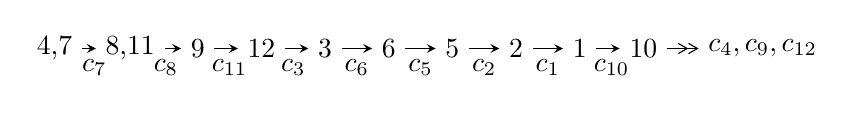
\begin{tikzpicture}[x=23pt, y=7pt]
	% node
	\node (A0) at (-1/8, 0) {4,7};
	\node (A1) at (17/16, 0) {8,11};
	\node (A2) at (17/8, 0) {9};
	\node (A3) at (25/8, 0) {12};
	\node (A4) at (33/8, 0) {3};
	\node (A5) at (41/8, 0) {6};
	\node (A6) at (49/8, 0) {5};
	\node (A7) at (57/8, 0) {2};
	\node (A8) at (65/8, 0) {1};
	\node (A9) at (73/8, 0) {10};
	\node (C1) at (1/2, -1) {$c_{7}$};
	\node (C2) at (13/8, -1) {$c_{8}$};
	\node (C3) at (21/8, -1) {$c_{11}$};
	\node (C4) at (29/8, -1) {$c_{3}$};
	\node (C5) at (37/8, -1) {$c_{6}$};
	\node (C6) at (45/8, -1) {$c_{5}$};
	\node (C7) at (53/8, -1) {$c_{2}$};
	\node (C8) at (61/8, -1) {$c_{1}$};
	\node (C9) at (69/8, -1) {$c_{10}$};
	\node (A10) at (11, 0) {$c_{4},c_{9},c_{12}$};

	% edge
	\draw[->,>=stealth]	
	(A0) edge (A1) (A1) edge (A2) (A2) edge (A3) (A3) edge (A4) (A4) edge (A5) (A5) edge (A6) (A6) edge (A7) (A7) edge (A8) (A8) edge (A9) ;
	\draw[->>,>={angle 60}]	
	(A9) edge (A10);
\end{tikzpicture} \\ 

\end{tabular} \\

\footnotetext{
The image of knot diagram is generated by the software ``\textbf{Draw programme}" developed by Andrew Bartholomew(\url{http://www.layer8.co.uk/maths/draw/index.htm\#Running-draw}), where we modified some parts for our purpose(\url{https://github.com/CATsTAILs/LinksPainter}).
}\phantom \\ \newline 
\centering \textbf{Ideals for irreducible components\footnotemark of $X_{\text{par}}$} 
 
\begin{align*}
I^u_{1}&=\langle 
1.03066\times10^{465} u^{124}+3.82536\times10^{465} u^{123}+\cdots+1.54622\times10^{467} b+1.91851\times10^{468},\\
\phantom{I^u_{1}}&\phantom{= \langle  }7.22439\times10^{466} u^{124}+2.12080\times10^{467} u^{123}+\cdots+2.31933\times10^{468} a+1.10931\times10^{470},\\
\phantom{I^u_{1}}&\phantom{= \langle  }u^{125}+2 u^{124}+\cdots+512 u+512\rangle \\
I^u_{2}&=\langle 
b,\;3 a+3 u-5,\;u^2- u-1\rangle \\
\\
I^v_{1}&=\langle 
a,\;16726 v^8-41423 v^7+\cdots+11959 b+26601,\\
\phantom{I^v_{1}}&\phantom{= \langle  }v^9-3 v^8-2 v^7-6 v^6+25 v^5-11 v^4-9 v^3+2 v^2+3 v-1\rangle \\
\end{align*}
\raggedright * 3 irreducible components of $\dim_{\mathbb{C}}=0$, with total 136 representations.\\
\footnotetext{All coefficients of polynomials are rational numbers. But the coefficients are sometimes approximated in decimal forms when there is not enough margin.}
\newpage
\renewcommand{\arraystretch}{1}
\centering \section*{I. $I^u_{1}= \langle 1.03\times10^{465} u^{124}+3.83\times10^{465} u^{123}+\cdots+1.55\times10^{467} b+1.92\times10^{468},\;7.22\times10^{466} u^{124}+2.12\times10^{467} u^{123}+\cdots+2.32\times10^{468} a+1.11\times10^{470},\;u^{125}+2 u^{124}+\cdots+512 u+512 \rangle$}
\flushleft \textbf{(i) Arc colorings}\\
\begin{tabular}{m{7pt} m{180pt} m{7pt} m{180pt} }
\flushright $a_{4}=$&$\begin{pmatrix}0\\u\end{pmatrix}$ \\
\flushright $a_{7}=$&$\begin{pmatrix}1\\0\end{pmatrix}$ \\
\flushright $a_{8}=$&$\begin{pmatrix}1\\u^2\end{pmatrix}$ \\
\flushright $a_{11}=$&$\begin{pmatrix}-0.0311487 u^{124}-0.0914405 u^{123}+\cdots-13.8068 u-47.8291\\-0.00666572 u^{124}-0.0247401 u^{123}+\cdots-5.19981 u-12.4077\end{pmatrix}$ \\
\flushright $a_{9}=$&$\begin{pmatrix}-0.0129299 u^{124}-0.0674498 u^{123}+\cdots+31.3986 u-57.3336\\0.00112353 u^{124}+0.0331708 u^{123}+\cdots-7.29416 u+30.7948\end{pmatrix}$ \\
\flushright $a_{12}=$&$\begin{pmatrix}-0.0378144 u^{124}-0.116181 u^{123}+\cdots-19.0066 u-60.2369\\-0.00666572 u^{124}-0.0247401 u^{123}+\cdots-5.19981 u-12.4077\end{pmatrix}$ \\
\flushright $a_{3}=$&$\begin{pmatrix}u\\u^3+u\end{pmatrix}$ \\
\flushright $a_{6}=$&$\begin{pmatrix}-0.0591666 u^{124}-0.127059 u^{123}+\cdots-50.3219 u-34.3988\\-0.0116249 u^{124}-0.0371386 u^{123}+\cdots+1.86792 u-26.7347\end{pmatrix}$ \\
\flushright $a_{5}=$&$\begin{pmatrix}-0.0241892 u^{124}-0.0463826 u^{123}+\cdots-18.7830 u-12.5336\\-0.0277806 u^{124}-0.0245777 u^{123}+\cdots-33.9805 u+8.02032\end{pmatrix}$ \\
\flushright $a_{2}=$&$\begin{pmatrix}-0.0165610 u^{124}+0.00694800 u^{123}+\cdots-26.5606 u+21.5758\\-0.0651205 u^{124}-0.0919181 u^{123}+\cdots-57.3802 u-11.4736\end{pmatrix}$ \\
\flushright $a_{1}=$&$\begin{pmatrix}-0.00359135 u^{124}+0.0218049 u^{123}+\cdots-15.1975 u+20.5539\\-0.0514815 u^{124}-0.0693144 u^{123}+\cdots-46.9834 u-6.82131\end{pmatrix}$ \\
\flushright $a_{10}=$&$\begin{pmatrix}-0.0277532 u^{124}-0.0756995 u^{123}+\cdots-20.2561 u-33.4474\\0.0514815 u^{124}+0.0693144 u^{123}+\cdots+46.9834 u+6.82131\end{pmatrix}$\\&\end{tabular}
\flushleft \textbf{(ii) Obstruction class $= -1$}\\~\\
\flushleft \textbf{(iii) Cusp Shapes $= -0.0955818 u^{124}-0.136137 u^{123}+\cdots-86.1084 u-11.1303$}\\~\\
\newpage\renewcommand{\arraystretch}{1}
\flushleft \textbf{(iv) u-Polynomials at the component}\newline \\
\begin{tabular}{m{50pt}|m{274pt}}
Crossings & \hspace{64pt}u-Polynomials at each crossing \\
\hline $$\begin{aligned}c_{1}\end{aligned}$$&$\begin{aligned}
&u^{125}+63 u^{124}+\cdots+271 u+1
\end{aligned}$\\
\hline $$\begin{aligned}c_{2},c_{4}\end{aligned}$$&$\begin{aligned}
&u^{125}-11 u^{124}+\cdots-9 u-1
\end{aligned}$\\
\hline $$\begin{aligned}c_{3},c_{7}\end{aligned}$$&$\begin{aligned}
&u^{125}+2 u^{124}+\cdots+512 u+512
\end{aligned}$\\
\hline $$\begin{aligned}c_{5}\end{aligned}$$&$\begin{aligned}
&9(9 u^{125}-12 u^{124}+\cdots+2.83664\times10^{9} u+2.59859\times10^{8})
\end{aligned}$\\
\hline $$\begin{aligned}c_{6},c_{9}\end{aligned}$$&$\begin{aligned}
&u^{125}-3 u^{124}+\cdots+3 u-1
\end{aligned}$\\
\hline $$\begin{aligned}c_{8}\end{aligned}$$&$\begin{aligned}
&9(9 u^{125}-21 u^{124}+\cdots+1.22889\times10^{8} u+5290529)
\end{aligned}$\\
\hline $$\begin{aligned}c_{10},c_{12}\end{aligned}$$&$\begin{aligned}
&u^{125}+4 u^{124}+\cdots-2358 u+81
\end{aligned}$\\
\hline $$\begin{aligned}c_{11}\end{aligned}$$&$\begin{aligned}
&u^{125}-2 u^{124}+\cdots-756 u+324
\end{aligned}$\\
\hline
\end{tabular}\\~\\
\newpage\renewcommand{\arraystretch}{1}
\flushleft \textbf{(v) Riley Polynomials at the component}\newline \\
\begin{tabular}{m{50pt}|m{274pt}}
Crossings & \hspace{64pt}Riley Polynomials at each crossing \\
\hline $$\begin{aligned}c_{1}\end{aligned}$$&$\begin{aligned}
&y^{125}+9 y^{124}+\cdots+91007 y-1
\end{aligned}$\\
\hline $$\begin{aligned}c_{2},c_{4}\end{aligned}$$&$\begin{aligned}
&y^{125}-63 y^{124}+\cdots+271 y-1
\end{aligned}$\\
\hline $$\begin{aligned}c_{3},c_{7}\end{aligned}$$&$\begin{aligned}
&y^{125}+54 y^{124}+\cdots-1572864 y-262144
\end{aligned}$\\
\hline $$\begin{aligned}c_{5}\end{aligned}$$&$\begin{aligned}
&81(81 y^{125}-3294 y^{124}+\cdots+2.87254\times10^{18} y-6.75265\times10^{16})
\end{aligned}$\\
\hline $$\begin{aligned}c_{6},c_{9}\end{aligned}$$&$\begin{aligned}
&y^{125}+85 y^{124}+\cdots+31 y-1
\end{aligned}$\\
\hline $$\begin{aligned}c_{8}\end{aligned}$$&$\begin{aligned}
&81\\
&\cdot(81 y^{125}-4023 y^{124}+\cdots+7567318376329835 y-27989697099841)
\end{aligned}$\\
\hline $$\begin{aligned}c_{10},c_{12}\end{aligned}$$&$\begin{aligned}
&y^{125}-90 y^{124}+\cdots+665982 y-6561
\end{aligned}$\\
\hline $$\begin{aligned}c_{11}\end{aligned}$$&$\begin{aligned}
&y^{125}-12 y^{124}+\cdots+16685352 y-104976
\end{aligned}$\\
\hline
\end{tabular}\\~\\
\newpage\flushleft \textbf{(vi) Complex Volumes and Cusp Shapes}
$$\begin{array}{c|c|c}  
\text{Solutions to }I^u_{1}& \I (\text{vol} + \sqrt{-1}CS) & \text{Cusp shape}\\
 \hline 
\begin{aligned}
u &= -0.189225 + 0.989929 I \\
a &= -2.72604 - 1.67999 I \\
b &= \phantom{-}0.545603 - 0.015975 I\end{aligned}
 & \phantom{-}4.85915 + 0.90928 I & \phantom{-0.000000 } 0 \\ \hline\begin{aligned}
u &= -0.189225 - 0.989929 I \\
a &= -2.72604 + 1.67999 I \\
b &= \phantom{-}0.545603 + 0.015975 I\end{aligned}
 & \phantom{-}4.85915 - 0.90928 I & \phantom{-0.000000 } 0 \\ \hline\begin{aligned}
u &= \phantom{-}0.913335 + 0.327879 I \\
a &= -0.13404 - 1.61461 I \\
b &= \phantom{-}1.42964 - 1.22199 I\end{aligned}
 & \phantom{-}4.24550 + 3.85404 I & \phantom{-0.000000 } 0 \\ \hline\begin{aligned}
u &= \phantom{-}0.913335 - 0.327879 I \\
a &= -0.13404 + 1.61461 I \\
b &= \phantom{-}1.42964 + 1.22199 I\end{aligned}
 & \phantom{-}4.24550 - 3.85404 I & \phantom{-0.000000 } 0 \\ \hline\begin{aligned}
u &= \phantom{-}0.532227 + 0.797562 I \\
a &= \phantom{-}1.88338 + 0.31904 I \\
b &= -0.465658 + 0.870917 I\end{aligned}
 & -4.18791 - 0.46329 I & \phantom{-0.000000 } 0 \\ \hline\begin{aligned}
u &= \phantom{-}0.532227 - 0.797562 I \\
a &= \phantom{-}1.88338 - 0.31904 I \\
b &= -0.465658 - 0.870917 I\end{aligned}
 & -4.18791 + 0.46329 I & \phantom{-0.000000 } 0 \\ \hline\begin{aligned}
u &= \phantom{-}0.495636 + 0.814877 I \\
a &= \phantom{-}0.168018 + 0.065540 I \\
b &= \phantom{-}0.221515 + 1.197440 I\end{aligned}
 & -4.15405 - 3.73457 I & \phantom{-0.000000 } 0 \\ \hline\begin{aligned}
u &= \phantom{-}0.495636 - 0.814877 I \\
a &= \phantom{-}0.168018 - 0.065540 I \\
b &= \phantom{-}0.221515 - 1.197440 I\end{aligned}
 & -4.15405 + 3.73457 I & \phantom{-0.000000 } 0 \\ \hline\begin{aligned}
u &= \phantom{-}0.080750 + 1.051060 I \\
a &= \phantom{-}1.320830 + 0.182380 I \\
b &= -0.932530 - 0.275816 I\end{aligned}
 & \phantom{-}2.33153 + 1.50993 I & \phantom{-0.000000 } 0 \\ \hline\begin{aligned}
u &= \phantom{-}0.080750 - 1.051060 I \\
a &= \phantom{-}1.320830 - 0.182380 I \\
b &= -0.932530 + 0.275816 I\end{aligned}
 & \phantom{-}2.33153 - 1.50993 I & \phantom{-0.000000 } 0\\
 \hline 
 \end{array}$$\newpage$$\begin{array}{c|c|c}  
\text{Solutions to }I^u_{1}& \I (\text{vol} + \sqrt{-1}CS) & \text{Cusp shape}\\
 \hline 
\begin{aligned}
u &= -0.413672 + 0.836934 I \\
a &= -0.275409 - 0.177834 I \\
b &= -0.74713 + 1.37671 I\end{aligned}
 & -0.983702 - 0.642828 I & \phantom{-0.000000 } 0 \\ \hline\begin{aligned}
u &= -0.413672 - 0.836934 I \\
a &= -0.275409 + 0.177834 I \\
b &= -0.74713 - 1.37671 I\end{aligned}
 & -0.983702 + 0.642828 I & \phantom{-0.000000 } 0 \\ \hline\begin{aligned}
u &= \phantom{-}0.918385 + 0.543413 I \\
a &= \phantom{-}0.240683 + 0.155590 I \\
b &= \phantom{-}0.604955 + 0.884379 I\end{aligned}
 & -3.67094 + 2.96823 I & \phantom{-0.000000 } 0 \\ \hline\begin{aligned}
u &= \phantom{-}0.918385 - 0.543413 I \\
a &= \phantom{-}0.240683 - 0.155590 I \\
b &= \phantom{-}0.604955 - 0.884379 I\end{aligned}
 & -3.67094 - 2.96823 I & \phantom{-0.000000 } 0 \\ \hline\begin{aligned}
u &= -0.422750 + 0.821064 I \\
a &= -3.17983 + 0.68595 I \\
b &= \phantom{-}1.19189 + 1.04668 I\end{aligned}
 & -1.03348 + 4.20848 I & \phantom{-0.000000 } 0 \\ \hline\begin{aligned}
u &= -0.422750 - 0.821064 I \\
a &= -3.17983 - 0.68595 I \\
b &= \phantom{-}1.19189 - 1.04668 I\end{aligned}
 & -1.03348 - 4.20848 I & \phantom{-0.000000 } 0 \\ \hline\begin{aligned}
u &= -0.962365 + 0.485559 I \\
a &= -0.437124 - 0.102030 I \\
b &= -1.34087 + 1.13393 I\end{aligned}
 & -0.31912 - 6.67340 I & \phantom{-0.000000 } 0 \\ \hline\begin{aligned}
u &= -0.962365 - 0.485559 I \\
a &= -0.437124 + 0.102030 I \\
b &= -1.34087 - 1.13393 I\end{aligned}
 & -0.31912 + 6.67340 I & \phantom{-0.000000 } 0 \\ \hline\begin{aligned}
u &= -0.807203 + 0.430889 I \\
a &= \phantom{-}0.056330 + 0.856214 I \\
b &= -0.364132 - 0.128397 I\end{aligned}
 & -0.121971 - 0.719876 I & \phantom{-0.000000 } 0 \\ \hline\begin{aligned}
u &= -0.807203 - 0.430889 I \\
a &= \phantom{-}0.056330 - 0.856214 I \\
b &= -0.364132 + 0.128397 I\end{aligned}
 & -0.121971 + 0.719876 I & \phantom{-0.000000 } 0\\
 \hline 
 \end{array}$$\newpage$$\begin{array}{c|c|c}  
\text{Solutions to }I^u_{1}& \I (\text{vol} + \sqrt{-1}CS) & \text{Cusp shape}\\
 \hline 
\begin{aligned}
u &= -0.828223 + 0.376343 I \\
a &= \phantom{-}1.21716 - 1.20280 I \\
b &= -0.702944 - 0.443518 I\end{aligned}
 & \phantom{-}0.06073 - 2.33875 I & \phantom{-0.000000 } 0 \\ \hline\begin{aligned}
u &= -0.828223 - 0.376343 I \\
a &= \phantom{-}1.21716 + 1.20280 I \\
b &= -0.702944 + 0.443518 I\end{aligned}
 & \phantom{-}0.06073 + 2.33875 I & \phantom{-0.000000 } 0 \\ \hline\begin{aligned}
u &= -0.599973 + 0.683518 I \\
a &= -0.077597 + 0.147796 I \\
b &= \phantom{-}0.471466 + 0.834279 I\end{aligned}
 & \phantom{-}1.14990 + 7.95106 I & \phantom{-0.000000 } 0 \\ \hline\begin{aligned}
u &= -0.599973 - 0.683518 I \\
a &= -0.077597 - 0.147796 I \\
b &= \phantom{-}0.471466 - 0.834279 I\end{aligned}
 & \phantom{-}1.14990 - 7.95106 I & \phantom{-0.000000 } 0 \\ \hline\begin{aligned}
u &= \phantom{-}0.402370 + 1.037470 I \\
a &= -0.86209 - 1.36616 I \\
b &= \phantom{-}0.498531 - 0.049477 I\end{aligned}
 & \phantom{-}3.98203 - 1.01780 I & \phantom{-0.000000 } 0 \\ \hline\begin{aligned}
u &= \phantom{-}0.402370 - 1.037470 I \\
a &= -0.86209 + 1.36616 I \\
b &= \phantom{-}0.498531 + 0.049477 I\end{aligned}
 & \phantom{-}3.98203 + 1.01780 I & \phantom{-0.000000 } 0 \\ \hline\begin{aligned}
u &= \phantom{-}1.090330 + 0.256832 I \\
a &= -0.0476149 + 0.1171240 I \\
b &= \phantom{-}1.10513 + 0.90387 I\end{aligned}
 & \phantom{-}6.12909 + 7.71732 I & \phantom{-0.000000 } 0 \\ \hline\begin{aligned}
u &= \phantom{-}1.090330 - 0.256832 I \\
a &= -0.0476149 - 0.1171240 I \\
b &= \phantom{-}1.10513 - 0.90387 I\end{aligned}
 & \phantom{-}6.12909 - 7.71732 I & \phantom{-0.000000 } 0 \\ \hline\begin{aligned}
u &= -0.248400 + 1.101470 I \\
a &= -1.33263 + 0.83830 I \\
b &= \phantom{-}0.354052 + 0.770723 I\end{aligned}
 & \phantom{-}4.76652 + 0.18641 I & \phantom{-0.000000 } 0 \\ \hline\begin{aligned}
u &= -0.248400 - 1.101470 I \\
a &= -1.33263 - 0.83830 I \\
b &= \phantom{-}0.354052 - 0.770723 I\end{aligned}
 & \phantom{-}4.76652 - 0.18641 I & \phantom{-0.000000 } 0\\
 \hline 
 \end{array}$$\newpage$$\begin{array}{c|c|c}  
\text{Solutions to }I^u_{1}& \I (\text{vol} + \sqrt{-1}CS) & \text{Cusp shape}\\
 \hline 
\begin{aligned}
u &= -0.433618 + 1.055720 I \\
a &= \phantom{-}2.35530 - 0.20832 I \\
b &= -1.11177 - 1.01672 I\end{aligned}
 & \phantom{-}3.54058 + 9.87816 I & \phantom{-0.000000 } 0 \\ \hline\begin{aligned}
u &= -0.433618 - 1.055720 I \\
a &= \phantom{-}2.35530 + 0.20832 I \\
b &= -1.11177 + 1.01672 I\end{aligned}
 & \phantom{-}3.54058 - 9.87816 I & \phantom{-0.000000 } 0 \\ \hline\begin{aligned}
u &= -0.442173 + 1.054840 I \\
a &= \phantom{-}1.210110 - 0.399870 I \\
b &= -1.063990 - 0.003120 I\end{aligned}
 & \phantom{-}1.15542 + 3.12032 I & \phantom{-0.000000 } 0 \\ \hline\begin{aligned}
u &= -0.442173 - 1.054840 I \\
a &= \phantom{-}1.210110 + 0.399870 I \\
b &= -1.063990 + 0.003120 I\end{aligned}
 & \phantom{-}1.15542 - 3.12032 I & \phantom{-0.000000 } 0 \\ \hline\begin{aligned}
u &= -0.840842 + 0.156626 I \\
a &= \phantom{-}0.52324 - 1.86364 I \\
b &= \phantom{-}0.84914 - 1.46811 I\end{aligned}
 & \phantom{-}4.74563 + 0.17252 I & \phantom{-}5.48395 + 0. I\phantom{ +0.000000I} \\ \hline\begin{aligned}
u &= -0.840842 - 0.156626 I \\
a &= \phantom{-}0.52324 + 1.86364 I \\
b &= \phantom{-}0.84914 + 1.46811 I\end{aligned}
 & \phantom{-}4.74563 - 0.17252 I & \phantom{-}5.48395 + 0. I\phantom{ +0.000000I} \\ \hline\begin{aligned}
u &= -0.064934 + 1.160180 I \\
a &= -1.74953 + 0.85168 I \\
b &= \phantom{-}1.73930 - 0.46575 I\end{aligned}
 & \phantom{-}5.99018 - 4.39123 I & \phantom{-0.000000 } 0 \\ \hline\begin{aligned}
u &= -0.064934 - 1.160180 I \\
a &= -1.74953 - 0.85168 I \\
b &= \phantom{-}1.73930 + 0.46575 I\end{aligned}
 & \phantom{-}5.99018 + 4.39123 I & \phantom{-0.000000 } 0 \\ \hline\begin{aligned}
u &= \phantom{-}0.380832 + 1.099280 I \\
a &= -1.49403 + 0.23024 I \\
b &= \phantom{-}0.649724 - 0.705708 I\end{aligned}
 & -1.50629 - 4.23005 I & \phantom{-0.000000 } 0 \\ \hline\begin{aligned}
u &= \phantom{-}0.380832 - 1.099280 I \\
a &= -1.49403 - 0.23024 I \\
b &= \phantom{-}0.649724 + 0.705708 I\end{aligned}
 & -1.50629 + 4.23005 I & \phantom{-0.000000 } 0\\
 \hline 
 \end{array}$$\newpage$$\begin{array}{c|c|c}  
\text{Solutions to }I^u_{1}& \I (\text{vol} + \sqrt{-1}CS) & \text{Cusp shape}\\
 \hline 
\begin{aligned}
u &= \phantom{-}0.349086 + 1.109990 I \\
a &= -1.222110 - 0.226288 I \\
b &= \phantom{-}0.746699 + 0.641099 I\end{aligned}
 & \phantom{-}4.36419 - 2.43164 I & \phantom{-0.000000 } 0 \\ \hline\begin{aligned}
u &= \phantom{-}0.349086 - 1.109990 I \\
a &= -1.222110 + 0.226288 I \\
b &= \phantom{-}0.746699 - 0.641099 I\end{aligned}
 & \phantom{-}4.36419 + 2.43164 I & \phantom{-0.000000 } 0 \\ \hline\begin{aligned}
u &= \phantom{-}0.375408 + 1.108420 I \\
a &= -1.25787 - 1.15535 I \\
b &= \phantom{-}1.85937 - 0.00043 I\end{aligned}
 & \phantom{-}5.08150 - 0.59588 I & \phantom{-0.000000 } 0 \\ \hline\begin{aligned}
u &= \phantom{-}0.375408 - 1.108420 I \\
a &= -1.25787 + 1.15535 I \\
b &= \phantom{-}1.85937 + 0.00043 I\end{aligned}
 & \phantom{-}5.08150 + 0.59588 I & \phantom{-0.000000 } 0 \\ \hline\begin{aligned}
u &= -0.235520 + 0.777319 I \\
a &= -0.153207 + 0.244390 I \\
b &= -0.262287 - 1.105520 I\end{aligned}
 & -0.40273 + 3.66473 I & \phantom{-0.000000 } 0. - 6.36269 I \\ \hline\begin{aligned}
u &= -0.235520 - 0.777319 I \\
a &= -0.153207 - 0.244390 I \\
b &= -0.262287 + 1.105520 I\end{aligned}
 & -0.40273 - 3.66473 I & \phantom{-0.000000 -}0. + 6.36269 I \\ \hline\begin{aligned}
u &= \phantom{-}1.112620 + 0.422938 I \\
a &= -0.0662946 - 0.1070030 I \\
b &= \phantom{-}0.823523 - 0.441900 I\end{aligned}
 & \phantom{-}5.54144 - 5.18578 I & \phantom{-0.000000 } 0 \\ \hline\begin{aligned}
u &= \phantom{-}1.112620 - 0.422938 I \\
a &= -0.0662946 + 0.1070030 I \\
b &= \phantom{-}0.823523 + 0.441900 I\end{aligned}
 & \phantom{-}5.54144 + 5.18578 I & \phantom{-0.000000 } 0 \\ \hline\begin{aligned}
u &= \phantom{-}0.523784 + 1.069500 I \\
a &= -4.10601 - 0.42204 I \\
b &= \phantom{-}0.376955 - 0.151157 I\end{aligned}
 & \phantom{-}3.20788 - 5.56394 I & \phantom{-0.000000 } 0 \\ \hline\begin{aligned}
u &= \phantom{-}0.523784 - 1.069500 I \\
a &= -4.10601 + 0.42204 I \\
b &= \phantom{-}0.376955 + 0.151157 I\end{aligned}
 & \phantom{-}3.20788 + 5.56394 I & \phantom{-0.000000 } 0\\
 \hline 
 \end{array}$$\newpage$$\begin{array}{c|c|c}  
\text{Solutions to }I^u_{1}& \I (\text{vol} + \sqrt{-1}CS) & \text{Cusp shape}\\
 \hline 
\begin{aligned}
u &= \phantom{-}0.634089 + 0.498710 I \\
a &= \phantom{-}3.69497 + 8.88764 I \\
b &= -0.145181 + 0.241855 I\end{aligned}
 & \phantom{-}1.42901 + 1.00847 I & -31.0649 + 44.2359 I \\ \hline\begin{aligned}
u &= \phantom{-}0.634089 - 0.498710 I \\
a &= \phantom{-}3.69497 - 8.88764 I \\
b &= -0.145181 - 0.241855 I\end{aligned}
 & \phantom{-}1.42901 - 1.00847 I & -31.0649 - 44.2359 I \\ \hline\begin{aligned}
u &= -0.505552 + 1.083710 I \\
a &= \phantom{-}1.41400 - 0.27693 I \\
b &= -0.785972 - 0.862103 I\end{aligned}
 & \phantom{-}0.63717 + 3.65490 I & \phantom{-0.000000 } 0 \\ \hline\begin{aligned}
u &= -0.505552 - 1.083710 I \\
a &= \phantom{-}1.41400 + 0.27693 I \\
b &= -0.785972 + 0.862103 I\end{aligned}
 & \phantom{-}0.63717 - 3.65490 I & \phantom{-0.000000 } 0 \\ \hline\begin{aligned}
u &= -1.185770 + 0.210987 I \\
a &= \phantom{-}0.0868843 - 0.0106217 I \\
b &= -0.608506 + 0.512349 I\end{aligned}
 & \phantom{-}0.98816 - 1.89695 I & \phantom{-0.000000 } 0 \\ \hline\begin{aligned}
u &= -1.185770 - 0.210987 I \\
a &= \phantom{-}0.0868843 + 0.0106217 I \\
b &= -0.608506 - 0.512349 I\end{aligned}
 & \phantom{-}0.98816 + 1.89695 I & \phantom{-0.000000 } 0 \\ \hline\begin{aligned}
u &= -0.666834 + 0.423916 I \\
a &= \phantom{-}0.286152 - 0.017589 I \\
b &= \phantom{-}0.257842 - 0.749663 I\end{aligned}
 & -1.37803 + 0.83267 I & -5.49260 - 3.40594 I \\ \hline\begin{aligned}
u &= -0.666834 - 0.423916 I \\
a &= \phantom{-}0.286152 + 0.017589 I \\
b &= \phantom{-}0.257842 + 0.749663 I\end{aligned}
 & -1.37803 - 0.83267 I & -5.49260 + 3.40594 I \\ \hline\begin{aligned}
u &= \phantom{-}0.234448 + 1.189590 I \\
a &= \phantom{-}1.74701 - 0.56723 I \\
b &= -1.01937 + 1.93388 I\end{aligned}
 & \phantom{-}9.39087 + 0.67963 I & \phantom{-0.000000 } 0 \\ \hline\begin{aligned}
u &= \phantom{-}0.234448 - 1.189590 I \\
a &= \phantom{-}1.74701 + 0.56723 I \\
b &= -1.01937 - 1.93388 I\end{aligned}
 & \phantom{-}9.39087 - 0.67963 I & \phantom{-0.000000 } 0\\
 \hline 
 \end{array}$$\newpage$$\begin{array}{c|c|c}  
\text{Solutions to }I^u_{1}& \I (\text{vol} + \sqrt{-1}CS) & \text{Cusp shape}\\
 \hline 
\begin{aligned}
u &= \phantom{-}0.750828 + 0.154017 I \\
a &= -0.540540 + 0.290736 I \\
b &= -1.094100 - 0.737261 I\end{aligned}
 & \phantom{-}1.33029 + 2.74208 I & \phantom{-}0.45355 - 2.62957 I \\ \hline\begin{aligned}
u &= \phantom{-}0.750828 - 0.154017 I \\
a &= -0.540540 - 0.290736 I \\
b &= -1.094100 + 0.737261 I\end{aligned}
 & \phantom{-}1.33029 - 2.74208 I & \phantom{-}0.45355 + 2.62957 I \\ \hline\begin{aligned}
u &= -0.360615 + 1.181320 I \\
a &= \phantom{-}0.77945 - 1.47555 I \\
b &= -1.65817 + 1.47843 I\end{aligned}
 & \phantom{-}8.85777 + 3.95009 I & \phantom{-0.000000 } 0 \\ \hline\begin{aligned}
u &= -0.360615 - 1.181320 I \\
a &= \phantom{-}0.77945 + 1.47555 I \\
b &= -1.65817 - 1.47843 I\end{aligned}
 & \phantom{-}8.85777 - 3.95009 I & \phantom{-0.000000 } 0 \\ \hline\begin{aligned}
u &= \phantom{-}0.521373 + 1.124290 I \\
a &= -0.96167 - 1.14782 I \\
b &= \phantom{-}0.202332 - 0.843758 I\end{aligned}
 & \phantom{-}3.12453 - 5.20896 I & \phantom{-0.000000 } 0 \\ \hline\begin{aligned}
u &= \phantom{-}0.521373 - 1.124290 I \\
a &= -0.96167 + 1.14782 I \\
b &= \phantom{-}0.202332 + 0.843758 I\end{aligned}
 & \phantom{-}3.12453 + 5.20896 I & \phantom{-0.000000 } 0 \\ \hline\begin{aligned}
u &= -1.124900 + 0.535801 I \\
a &= -0.0411915 - 0.1178360 I \\
b &= \phantom{-}1.16484 - 1.07257 I\end{aligned}
 & \phantom{-}4.42812 - 12.73300 I & \phantom{-0.000000 } 0 \\ \hline\begin{aligned}
u &= -1.124900 - 0.535801 I \\
a &= -0.0411915 + 0.1178360 I \\
b &= \phantom{-}1.16484 + 1.07257 I\end{aligned}
 & \phantom{-}4.42812 + 12.73300 I & \phantom{-0.000000 } 0 \\ \hline\begin{aligned}
u &= \phantom{-}0.492797 + 1.146900 I \\
a &= -2.03102 - 0.36281 I \\
b &= \phantom{-}1.54887 - 1.18166 I\end{aligned}
 & \phantom{-}4.19431 - 7.27901 I & \phantom{-0.000000 } 0 \\ \hline\begin{aligned}
u &= \phantom{-}0.492797 - 1.146900 I \\
a &= -2.03102 + 0.36281 I \\
b &= \phantom{-}1.54887 + 1.18166 I\end{aligned}
 & \phantom{-}4.19431 + 7.27901 I & \phantom{-0.000000 } 0\\
 \hline 
 \end{array}$$\newpage$$\begin{array}{c|c|c}  
\text{Solutions to }I^u_{1}& \I (\text{vol} + \sqrt{-1}CS) & \text{Cusp shape}\\
 \hline 
\begin{aligned}
u &= -0.615779 + 1.088750 I \\
a &= -0.650976 + 1.024930 I \\
b &= \phantom{-}0.414729 + 0.215546 I\end{aligned}
 & \phantom{-}1.80618 + 5.96754 I & \phantom{-0.000000 } 0 \\ \hline\begin{aligned}
u &= -0.615779 - 1.088750 I \\
a &= -0.650976 - 1.024930 I \\
b &= \phantom{-}0.414729 - 0.215546 I\end{aligned}
 & \phantom{-}1.80618 - 5.96754 I & \phantom{-0.000000 } 0 \\ \hline\begin{aligned}
u &= \phantom{-}0.699810 + 0.253258 I \\
a &= \phantom{-}0.45949 - 2.64155 I \\
b &= -0.233666 - 0.523885 I\end{aligned}
 & \phantom{-}0.621061 + 0.585081 I & -8.38094 - 6.55158 I \\ \hline\begin{aligned}
u &= \phantom{-}0.699810 - 0.253258 I \\
a &= \phantom{-}0.45949 + 2.64155 I \\
b &= -0.233666 + 0.523885 I\end{aligned}
 & \phantom{-}0.621061 - 0.585081 I & -8.38094 + 6.55158 I \\ \hline\begin{aligned}
u &= \phantom{-}1.156140 + 0.507162 I \\
a &= \phantom{-}0.0934185 - 0.0006937 I \\
b &= -0.757298 - 0.778048 I\end{aligned}
 & -0.51148 + 7.10641 I & \phantom{-0.000000 } 0 \\ \hline\begin{aligned}
u &= \phantom{-}1.156140 - 0.507162 I \\
a &= \phantom{-}0.0934185 + 0.0006937 I \\
b &= -0.757298 + 0.778048 I\end{aligned}
 & -0.51148 - 7.10641 I & \phantom{-0.000000 } 0 \\ \hline\begin{aligned}
u &= -0.329817 + 0.655522 I \\
a &= \phantom{-}0.27779 + 2.85032 I \\
b &= \phantom{-}0.435012 - 0.387028 I\end{aligned}
 & -0.74776 - 1.32568 I & -1.37223 - 2.12566 I \\ \hline\begin{aligned}
u &= -0.329817 - 0.655522 I \\
a &= \phantom{-}0.27779 - 2.85032 I \\
b &= \phantom{-}0.435012 + 0.387028 I\end{aligned}
 & -0.74776 + 1.32568 I & -1.37223 + 2.12566 I \\ \hline\begin{aligned}
u &= -0.585773 + 1.136850 I \\
a &= \phantom{-}0.270868 - 0.774974 I \\
b &= -0.675543 + 0.280117 I\end{aligned}
 & \phantom{-}2.57218 - 2.94748 I & \phantom{-0.000000 } 0 \\ \hline\begin{aligned}
u &= -0.585773 - 1.136850 I \\
a &= \phantom{-}0.270868 + 0.774974 I \\
b &= -0.675543 - 0.280117 I\end{aligned}
 & \phantom{-}2.57218 + 2.94748 I & \phantom{-0.000000 } 0\\
 \hline 
 \end{array}$$\newpage$$\begin{array}{c|c|c}  
\text{Solutions to }I^u_{1}& \I (\text{vol} + \sqrt{-1}CS) & \text{Cusp shape}\\
 \hline 
\begin{aligned}
u &= \phantom{-}0.164951 + 0.699060 I \\
a &= \phantom{-}2.01057 + 3.83403 I \\
b &= -1.12027 - 1.11356 I\end{aligned}
 & \phantom{-}3.23791 - 1.80187 I & \phantom{-}7.60062 + 5.39442 I \\ \hline\begin{aligned}
u &= \phantom{-}0.164951 - 0.699060 I \\
a &= \phantom{-}2.01057 - 3.83403 I \\
b &= -1.12027 + 1.11356 I\end{aligned}
 & \phantom{-}3.23791 + 1.80187 I & \phantom{-}7.60062 - 5.39442 I \\ \hline\begin{aligned}
u &= -0.494783 + 1.183550 I \\
a &= \phantom{-}1.67549 + 0.02049 I \\
b &= -0.72180 - 2.14415 I\end{aligned}
 & \phantom{-}7.89707 + 4.62521 I & \phantom{-0.000000 } 0 \\ \hline\begin{aligned}
u &= -0.494783 - 1.183550 I \\
a &= \phantom{-}1.67549 - 0.02049 I \\
b &= -0.72180 + 2.14415 I\end{aligned}
 & \phantom{-}7.89707 - 4.62521 I & \phantom{-0.000000 } 0 \\ \hline\begin{aligned}
u &= -0.581083 + 1.144450 I \\
a &= -0.927414 + 0.371926 I \\
b &= \phantom{-}0.912764 - 0.614051 I\end{aligned}
 & \phantom{-}2.41939 + 7.59298 I & \phantom{-0.000000 } 0 \\ \hline\begin{aligned}
u &= -0.581083 - 1.144450 I \\
a &= -0.927414 - 0.371926 I \\
b &= \phantom{-}0.912764 + 0.614051 I\end{aligned}
 & \phantom{-}2.41939 - 7.59298 I & \phantom{-0.000000 } 0 \\ \hline\begin{aligned}
u &= \phantom{-}0.277864 + 0.645271 I \\
a &= \phantom{-}0.1293420 - 0.0177373 I \\
b &= -0.259855 - 1.133830 I\end{aligned}
 & -3.17582 + 1.37189 I & -2.02901 + 3.10189 I \\ \hline\begin{aligned}
u &= \phantom{-}0.277864 - 0.645271 I \\
a &= \phantom{-}0.1293420 + 0.0177373 I \\
b &= -0.259855 + 1.133830 I\end{aligned}
 & -3.17582 - 1.37189 I & -2.02901 - 3.10189 I \\ \hline\begin{aligned}
u &= -0.349910 + 0.596945 I \\
a &= -0.044338 - 0.135561 I \\
b &= \phantom{-}0.776083 - 1.123390 I\end{aligned}
 & \phantom{-}1.92234 - 6.42207 I & \phantom{-}1.61043 - 2.58323 I \\ \hline\begin{aligned}
u &= -0.349910 - 0.596945 I \\
a &= -0.044338 + 0.135561 I \\
b &= \phantom{-}0.776083 + 1.123390 I\end{aligned}
 & \phantom{-}1.92234 + 6.42207 I & \phantom{-}1.61043 + 2.58323 I\\
 \hline 
 \end{array}$$\newpage$$\begin{array}{c|c|c}  
\text{Solutions to }I^u_{1}& \I (\text{vol} + \sqrt{-1}CS) & \text{Cusp shape}\\
 \hline 
\begin{aligned}
u &= \phantom{-}0.675342 + 0.102623 I \\
a &= -0.475944 - 0.632806 I \\
b &= -0.798997 + 0.456385 I\end{aligned}
 & \phantom{-}1.33240 - 2.49877 I & \phantom{-}0.06108 + 4.74869 I \\ \hline\begin{aligned}
u &= \phantom{-}0.675342 - 0.102623 I \\
a &= -0.475944 + 0.632806 I \\
b &= -0.798997 - 0.456385 I\end{aligned}
 & \phantom{-}1.33240 + 2.49877 I & \phantom{-}0.06108 - 4.74869 I \\ \hline\begin{aligned}
u &= \phantom{-}0.675422 + 1.130710 I \\
a &= \phantom{-}1.322000 + 0.441156 I \\
b &= -0.812816 + 1.037590 I\end{aligned}
 & -1.80399 - 8.86816 I & \phantom{-0.000000 } 0 \\ \hline\begin{aligned}
u &= \phantom{-}0.675422 - 1.130710 I \\
a &= \phantom{-}1.322000 - 0.441156 I \\
b &= -0.812816 - 1.037590 I\end{aligned}
 & -1.80399 + 8.86816 I & \phantom{-0.000000 } 0 \\ \hline\begin{aligned}
u &= \phantom{-}0.585027 + 1.188980 I \\
a &= \phantom{-}0.35499 + 1.37574 I \\
b &= -1.89934 - 1.32123 I\end{aligned}
 & \phantom{-}6.93778 - 9.34093 I & \phantom{-0.000000 } 0 \\ \hline\begin{aligned}
u &= \phantom{-}0.585027 - 1.188980 I \\
a &= \phantom{-}0.35499 - 1.37574 I \\
b &= -1.89934 + 1.32123 I\end{aligned}
 & \phantom{-}6.93778 + 9.34093 I & \phantom{-0.000000 } 0 \\ \hline\begin{aligned}
u &= -0.670642 + 1.165170 I \\
a &= -1.78726 + 0.65220 I \\
b &= \phantom{-}1.52212 + 1.38459 I\end{aligned}
 & \phantom{-}1.83437 + 12.66320 I & \phantom{-0.000000 } 0 \\ \hline\begin{aligned}
u &= -0.670642 - 1.165170 I \\
a &= -1.78726 - 0.65220 I \\
b &= \phantom{-}1.52212 - 1.38459 I\end{aligned}
 & \phantom{-}1.83437 - 12.66320 I & \phantom{-0.000000 } 0 \\ \hline\begin{aligned}
u &= -1.212360 + 0.646222 I \\
a &= -0.0620166 + 0.0911191 I \\
b &= \phantom{-}0.676884 + 0.094872 I\end{aligned}
 & \phantom{-}3.33646 - 0.19030 I & \phantom{-0.000000 } 0 \\ \hline\begin{aligned}
u &= -1.212360 - 0.646222 I \\
a &= -0.0620166 - 0.0911191 I \\
b &= \phantom{-}0.676884 - 0.094872 I\end{aligned}
 & \phantom{-}3.33646 + 0.19030 I & \phantom{-0.000000 } 0\\
 \hline 
 \end{array}$$\newpage$$\begin{array}{c|c|c}  
\text{Solutions to }I^u_{1}& \I (\text{vol} + \sqrt{-1}CS) & \text{Cusp shape}\\
 \hline 
\begin{aligned}
u &= -0.327090 + 0.526695 I \\
a &= -2.03892 + 2.29943 I \\
b &= \phantom{-}0.609994 - 0.249849 I\end{aligned}
 & -0.596246 + 0.416978 I & \phantom{-}0.26642 - 6.11778 I \\ \hline\begin{aligned}
u &= -0.327090 - 0.526695 I \\
a &= -2.03892 - 2.29943 I \\
b &= \phantom{-}0.609994 + 0.249849 I\end{aligned}
 & -0.596246 - 0.416978 I & \phantom{-}0.26642 + 6.11778 I \\ \hline\begin{aligned}
u &= \phantom{-}0.612331 + 1.251960 I \\
a &= \phantom{-}1.73548 + 0.43034 I \\
b &= -1.25293 + 1.11281 I\end{aligned}
 & \phantom{-}9.2901 - 13.7168 I & \phantom{-0.000000 } 0 \\ \hline\begin{aligned}
u &= \phantom{-}0.612331 - 1.251960 I \\
a &= \phantom{-}1.73548 - 0.43034 I \\
b &= -1.25293 - 1.11281 I\end{aligned}
 & \phantom{-}9.2901 + 13.7168 I & \phantom{-0.000000 } 0 \\ \hline\begin{aligned}
u &= -0.60524 + 1.28225 I \\
a &= -1.283780 + 0.186550 I \\
b &= \phantom{-}0.904103 + 0.810181 I\end{aligned}
 & \phantom{-}4.45793 + 8.07080 I & \phantom{-0.000000 } 0 \\ \hline\begin{aligned}
u &= -0.60524 - 1.28225 I \\
a &= -1.283780 - 0.186550 I \\
b &= \phantom{-}0.904103 - 0.810181 I\end{aligned}
 & \phantom{-}4.45793 - 8.07080 I & \phantom{-0.000000 } 0 \\ \hline\begin{aligned}
u &= -0.75455 + 1.21679 I \\
a &= \phantom{-}1.62826 - 0.67265 I \\
b &= -1.23586 - 1.20855 I\end{aligned}
 & \phantom{-}6.6329 + 19.4885 I & \phantom{-0.000000 } 0 \\ \hline\begin{aligned}
u &= -0.75455 - 1.21679 I \\
a &= \phantom{-}1.62826 + 0.67265 I \\
b &= -1.23586 + 1.20855 I\end{aligned}
 & \phantom{-}6.6329 - 19.4885 I & \phantom{-0.000000 } 0 \\ \hline\begin{aligned}
u &= \phantom{-}0.07864 + 1.43412 I \\
a &= \phantom{-}1.38519 - 0.43108 I \\
b &= -1.30927 + 0.70376 I\end{aligned}
 & \phantom{-}12.5560 - 9.3062 I & \phantom{-0.000000 } 0 \\ \hline\begin{aligned}
u &= \phantom{-}0.07864 - 1.43412 I \\
a &= \phantom{-}1.38519 + 0.43108 I \\
b &= -1.30927 - 0.70376 I\end{aligned}
 & \phantom{-}12.5560 + 9.3062 I & \phantom{-0.000000 } 0\\
 \hline 
 \end{array}$$\newpage$$\begin{array}{c|c|c}  
\text{Solutions to }I^u_{1}& \I (\text{vol} + \sqrt{-1}CS) & \text{Cusp shape}\\
 \hline 
\begin{aligned}
u &= \phantom{-}0.75063 + 1.23502 I \\
a &= -1.301480 - 0.365678 I \\
b &= \phantom{-}0.913051 - 0.950042 I\end{aligned}
 & \phantom{-}1.84566 - 13.92260 I & \phantom{-0.000000 } 0 \\ \hline\begin{aligned}
u &= \phantom{-}0.75063 - 1.23502 I \\
a &= -1.301480 + 0.365678 I \\
b &= \phantom{-}0.913051 + 0.950042 I\end{aligned}
 & \phantom{-}1.84566 + 13.92260 I & \phantom{-0.000000 } 0 \\ \hline\begin{aligned}
u &= \phantom{-}0.15570 + 1.44249 I \\
a &= \phantom{-}1.116080 + 0.615912 I \\
b &= -1.255060 - 0.503238 I\end{aligned}
 & \phantom{-}12.41370 + 3.14260 I & \phantom{-0.000000 } 0 \\ \hline\begin{aligned}
u &= \phantom{-}0.15570 - 1.44249 I \\
a &= \phantom{-}1.116080 - 0.615912 I \\
b &= -1.255060 + 0.503238 I\end{aligned}
 & \phantom{-}12.41370 - 3.14260 I & \phantom{-0.000000 } 0 \\ \hline\begin{aligned}
u &= -0.546681\phantom{ +0.000000I} \\
a &= \phantom{-}0.853690\phantom{ +0.000000I} \\
b &= \phantom{-}0.327961\phantom{ +0.000000I}\end{aligned}
 & -1.13268\phantom{ +0.000000I} & -9.63470\phantom{ +0.000000I} \\ \hline\begin{aligned}
u &= \phantom{-}0.69181 + 1.30600 I \\
a &= \phantom{-}0.556692 + 0.479724 I \\
b &= -0.828035 + 0.099208 I\end{aligned}
 & \phantom{-}8.30974 - 1.49559 I & \phantom{-0.000000 } 0 \\ \hline\begin{aligned}
u &= \phantom{-}0.69181 - 1.30600 I \\
a &= \phantom{-}0.556692 - 0.479724 I \\
b &= -0.828035 - 0.099208 I\end{aligned}
 & \phantom{-}8.30974 + 1.49559 I & \phantom{-0.000000 } 0 \\ \hline\begin{aligned}
u &= -0.79848 + 1.26772 I \\
a &= \phantom{-}0.617339 - 0.371174 I \\
b &= -0.753084 - 0.344913 I\end{aligned}
 & \phantom{-}5.49346 + 7.52898 I & \phantom{-0.000000 } 0 \\ \hline\begin{aligned}
u &= -0.79848 - 1.26772 I \\
a &= \phantom{-}0.617339 + 0.371174 I \\
b &= -0.753084 + 0.344913 I\end{aligned}
 & \phantom{-}5.49346 - 7.52898 I & \phantom{-0.000000 } 0 \\ \hline\begin{aligned}
u &= -0.09910 + 1.49843 I \\
a &= -0.912897 - 0.029897 I \\
b &= \phantom{-}0.928225 + 0.156147 I\end{aligned}
 & \phantom{-}7.75260 + 3.19534 I & \phantom{-0.000000 } 0\\
 \hline 
 \end{array}$$\newpage$$\begin{array}{c|c|c}  
\text{Solutions to }I^u_{1}& \I (\text{vol} + \sqrt{-1}CS) & \text{Cusp shape}\\
 \hline 
\begin{aligned}
u &= -0.09910 - 1.49843 I \\
a &= -0.912897 + 0.029897 I \\
b &= \phantom{-}0.928225 - 0.156147 I\end{aligned}
 & \phantom{-}7.75260 - 3.19534 I & \phantom{-0.000000 } 0 \\ \hline\begin{aligned}
u &= -0.234925 + 0.344834 I \\
a &= -0.39694 - 3.35327 I \\
b &= \phantom{-}0.591198 - 0.673652 I\end{aligned}
 & \phantom{-}4.30327 + 1.14568 I & \phantom{-}3.56993 + 0.21405 I \\ \hline\begin{aligned}
u &= -0.234925 - 0.344834 I \\
a &= -0.39694 + 3.35327 I \\
b &= \phantom{-}0.591198 + 0.673652 I\end{aligned}
 & \phantom{-}4.30327 - 1.14568 I & \phantom{-}3.56993 - 0.21405 I \\ \hline\begin{aligned}
u &= \phantom{-}1.62729\phantom{ +0.000000I} \\
a &= \phantom{-}0.0237227\phantom{ +0.000000I} \\
b &= -0.0964470\phantom{ +0.000000I}\end{aligned}
 & -7.22833\phantom{ +0.000000I} & \phantom{-0.000000 } 0 \\ \hline\begin{aligned}
u &= \phantom{-}0.239647\phantom{ +0.000000I} \\
a &= \phantom{-}3.21183\phantom{ +0.000000I} \\
b &= -0.449696\phantom{ +0.000000I}\end{aligned}
 & \phantom{-}1.26613\phantom{ +0.000000I} & \phantom{-}9.42890\phantom{ +0.000000I}\\
 \hline 
 \end{array}$$\newpage\newpage\renewcommand{\arraystretch}{1}
\centering \section*{II. $I^u_{2}= \langle b,\;3 a+3 u-5,\;u^2- u-1 \rangle$}
\flushleft \textbf{(i) Arc colorings}\\
\begin{tabular}{m{7pt} m{180pt} m{7pt} m{180pt} }
\flushright $a_{4}=$&$\begin{pmatrix}0\\u\end{pmatrix}$ \\
\flushright $a_{7}=$&$\begin{pmatrix}1\\0\end{pmatrix}$ \\
\flushright $a_{8}=$&$\begin{pmatrix}1\\u+1\end{pmatrix}$ \\
\flushright $a_{11}=$&$\begin{pmatrix}- u+\frac{5}{3}\\0\end{pmatrix}$ \\
\flushright $a_{9}=$&$\begin{pmatrix}-\frac{8}{9} u+\frac{22}{9}\\u+1\end{pmatrix}$ \\
\flushright $a_{12}=$&$\begin{pmatrix}- u+\frac{5}{3}\\0\end{pmatrix}$ \\
\flushright $a_{3}=$&$\begin{pmatrix}u\\3 u+1\end{pmatrix}$ \\
\flushright $a_{6}=$&$\begin{pmatrix}-\frac{2}{3} u-\frac{5}{9}\\-3 u-2\end{pmatrix}$ \\
\flushright $a_{5}=$&$\begin{pmatrix}- u\\-3 u-2\end{pmatrix}$ \\
\flushright $a_{2}=$&$\begin{pmatrix}-1\\-2 u-2\end{pmatrix}$ \\
\flushright $a_{1}=$&$\begin{pmatrix}-2 u-2\\-9 u-6\end{pmatrix}$ \\
\flushright $a_{10}=$&$\begin{pmatrix}u+\frac{11}{3}\\9 u+6\end{pmatrix}$\\&\end{tabular}
\flushleft \textbf{(ii) Obstruction class $= 1$}\\~\\
\flushleft \textbf{(iii) Cusp Shapes $= -\frac{560}{3} u-\frac{1105}{9}$}\\~\\
\newpage\renewcommand{\arraystretch}{1}
\flushleft \textbf{(iv) u-Polynomials at the component}\newline \\
\begin{tabular}{m{50pt}|m{274pt}}
Crossings & \hspace{64pt}u-Polynomials at each crossing \\
\hline $$\begin{aligned}c_{1},c_{6}\end{aligned}$$&$\begin{aligned}
&u^2-3 u+1
\end{aligned}$\\
\hline $$\begin{aligned}c_{2},c_{3}\end{aligned}$$&$\begin{aligned}
&u^2+u-1
\end{aligned}$\\
\hline $$\begin{aligned}c_{4},c_{7}\end{aligned}$$&$\begin{aligned}
&u^2- u-1
\end{aligned}$\\
\hline $$\begin{aligned}c_{5}\end{aligned}$$&$\begin{aligned}
&(3 u-1)^2
\end{aligned}$\\
\hline $$\begin{aligned}c_{8}\end{aligned}$$&$\begin{aligned}
&9 u^2+9 u+1
\end{aligned}$\\
\hline $$\begin{aligned}c_{9}\end{aligned}$$&$\begin{aligned}
&u^2+3 u+1
\end{aligned}$\\
\hline $$\begin{aligned}c_{10}\end{aligned}$$&$\begin{aligned}
&(u+1)^2
\end{aligned}$\\
\hline $$\begin{aligned}c_{11}\end{aligned}$$&$\begin{aligned}
&u^2
\end{aligned}$\\
\hline $$\begin{aligned}c_{12}\end{aligned}$$&$\begin{aligned}
&(u-1)^2
\end{aligned}$\\
\hline
\end{tabular}\\~\\
\newpage\renewcommand{\arraystretch}{1}
\flushleft \textbf{(v) Riley Polynomials at the component}\newline \\
\begin{tabular}{m{50pt}|m{274pt}}
Crossings & \hspace{64pt}Riley Polynomials at each crossing \\
\hline $$\begin{aligned}c_{1},c_{6},c_{9}\end{aligned}$$&$\begin{aligned}
&y^2-7 y+1
\end{aligned}$\\
\hline $$\begin{aligned}c_{2},c_{3},c_{4}\\c_{7}\end{aligned}$$&$\begin{aligned}
&y^2-3 y+1
\end{aligned}$\\
\hline $$\begin{aligned}c_{5}\end{aligned}$$&$\begin{aligned}
&(9 y-1)^2
\end{aligned}$\\
\hline $$\begin{aligned}c_{8}\end{aligned}$$&$\begin{aligned}
&81 y^2-63 y+1
\end{aligned}$\\
\hline $$\begin{aligned}c_{10},c_{12}\end{aligned}$$&$\begin{aligned}
&(y-1)^2
\end{aligned}$\\
\hline $$\begin{aligned}c_{11}\end{aligned}$$&$\begin{aligned}
&y^2
\end{aligned}$\\
\hline
\end{tabular}\\~\\
\newpage\flushleft \textbf{(vi) Complex Volumes and Cusp Shapes}
$$\begin{array}{c|c|c}  
\text{Solutions to }I^u_{2}& \I (\text{vol} + \sqrt{-1}CS) & \text{Cusp shape}\\
 \hline 
\begin{aligned}
u &= -0.618034\phantom{ +0.000000I} \\
a &= \phantom{-}2.28470\phantom{ +0.000000I} \\
b &= \phantom{-0.000000 } 0\end{aligned}
 & \phantom{-}0.657974\phantom{ +0.000000I} & -7.41140\phantom{ +0.000000I} \\ \hline\begin{aligned}
u &= \phantom{-}1.61803\phantom{ +0.000000I} \\
a &= \phantom{-}0.0486327\phantom{ +0.000000I} \\
b &= \phantom{-0.000000 } 0\end{aligned}
 & -7.23771\phantom{ +0.000000I} & -424.810\phantom{ +0.000000I}\\
 \hline 
 \end{array}$$\newpage\newpage\renewcommand{\arraystretch}{1}
\centering \section*{III. $I^v_{1}= \langle a,\;16726 v^8-41423 v^7+\cdots+11959 b+26601,\;v^9-3 v^8+\cdots+3 v-1 \rangle$}
\flushleft \textbf{(i) Arc colorings}\\
\begin{tabular}{m{7pt} m{180pt} m{7pt} m{180pt} }
\flushright $a_{4}=$&$\begin{pmatrix}v\\0\end{pmatrix}$ \\
\flushright $a_{7}=$&$\begin{pmatrix}1\\0\end{pmatrix}$ \\
\flushright $a_{8}=$&$\begin{pmatrix}1\\0\end{pmatrix}$ \\
\flushright $a_{11}=$&$\begin{pmatrix}0\\-1.39861 v^{8}+3.46375 v^{7}+\cdots+3.94598 v-2.22435\end{pmatrix}$ \\
\flushright $a_{9}=$&$\begin{pmatrix}1\\1.45213 v^{8}-3.82515 v^{7}+\cdots-3.73944 v+4.14098\end{pmatrix}$ \\
\flushright $a_{12}=$&$\begin{pmatrix}-1.39861 v^{8}+3.46375 v^{7}+\cdots+3.94598 v-2.22435\\-1.39861 v^{8}+3.46375 v^{7}+\cdots+3.94598 v-2.22435\end{pmatrix}$ \\
\flushright $a_{3}=$&$\begin{pmatrix}v\\0\end{pmatrix}$ \\
\flushright $a_{6}=$&$\begin{pmatrix}-1.45213 v^{8}+3.82515 v^{7}+\cdots+3.73944 v-3.14098\\-1.21114 v^{8}+2.94147 v^{7}+\cdots+5.63826 v-2.00702\end{pmatrix}$ \\
\flushright $a_{5}=$&$\begin{pmatrix}0.759010 v^{8}-2.11631 v^{7}+\cdots+0.101179 v+1.86604\\v^8-3 v^7-2 v^6-6 v^5+25 v^4-11 v^3-9 v^2+2 v+3\end{pmatrix}$ \\
\flushright $a_{2}=$&$\begin{pmatrix}-0.759010 v^{8}+2.11631 v^{7}+\cdots+0.898821 v-1.86604\\- v^8+3 v^7+2 v^6+6 v^5-25 v^4+11 v^3+9 v^2-2 v-3\end{pmatrix}$ \\
\flushright $a_{1}=$&$\begin{pmatrix}-0.759010 v^{8}+2.11631 v^{7}+\cdots-0.101179 v-1.86604\\- v^8+3 v^7+2 v^6+6 v^5-25 v^4+11 v^3+9 v^2-2 v-3\end{pmatrix}$ \\
\flushright $a_{10}=$&$\begin{pmatrix}-0.240990 v^{8}+0.883686 v^{7}+\cdots-1.89882 v-1.13396\\- v^8+3 v^7+2 v^6+6 v^5-25 v^4+11 v^3+9 v^2-2 v-3\end{pmatrix}$\\&\end{tabular}
\flushleft \textbf{(ii) Obstruction class $= 1$}\\~\\
\flushleft \textbf{(iii) Cusp Shapes $= \frac{109765}{11959} v^8-\frac{294476}{11959} v^7-\frac{325323}{11959} v^6-\frac{729072}{11959} v^5+\frac{2542695}{11959} v^4-\frac{295872}{11959} v^3-\frac{1329263}{11959} v^2-\frac{115465}{11959} v+\frac{259811}{11959}$}\\~\\
\newpage\renewcommand{\arraystretch}{1}
\flushleft \textbf{(iv) u-Polynomials at the component}\newline \\
\begin{tabular}{m{50pt}|m{274pt}}
Crossings & \hspace{64pt}u-Polynomials at each crossing \\
\hline $$\begin{aligned}c_{1},c_{2}\end{aligned}$$&$\begin{aligned}
&(u-1)^9
\end{aligned}$\\
\hline $$\begin{aligned}c_{3},c_{7}\end{aligned}$$&$\begin{aligned}
&u^9
\end{aligned}$\\
\hline $$\begin{aligned}c_{4}\end{aligned}$$&$\begin{aligned}
&(u+1)^9
\end{aligned}$\\
\hline $$\begin{aligned}c_{5}\end{aligned}$$&$\begin{aligned}
&u^9+5 u^8+12 u^7+15 u^6+9 u^5- u^4-4 u^3-2 u^2+u+1
\end{aligned}$\\
\hline $$\begin{aligned}c_{6}\end{aligned}$$&$\begin{aligned}
&u^9-3 u^8+8 u^7-13 u^6+17 u^5-17 u^4+12 u^3-6 u^2+u+1
\end{aligned}$\\
\hline $$\begin{aligned}c_{8}\end{aligned}$$&$\begin{aligned}
&u^9- u^8+2 u^7- u^6+3 u^5- u^4+2 u^3+u+1
\end{aligned}$\\
\hline $$\begin{aligned}c_{9}\end{aligned}$$&$\begin{aligned}
&u^9+3 u^8+8 u^7+13 u^6+17 u^5+17 u^4+12 u^3+6 u^2+u-1
\end{aligned}$\\
\hline $$\begin{aligned}c_{10}\end{aligned}$$&$\begin{aligned}
&u^9- u^8-2 u^7+3 u^6+u^5-3 u^4+2 u^3- u+1
\end{aligned}$\\
\hline $$\begin{aligned}c_{11}\end{aligned}$$&$\begin{aligned}
&u^9+u^8+2 u^7+u^6+3 u^5+u^4+2 u^3+u-1
\end{aligned}$\\
\hline $$\begin{aligned}c_{12}\end{aligned}$$&$\begin{aligned}
&u^9+u^8-2 u^7-3 u^6+u^5+3 u^4+2 u^3- u-1
\end{aligned}$\\
\hline
\end{tabular}\\~\\
\newpage\renewcommand{\arraystretch}{1}
\flushleft \textbf{(v) Riley Polynomials at the component}\newline \\
\begin{tabular}{m{50pt}|m{274pt}}
Crossings & \hspace{64pt}Riley Polynomials at each crossing \\
\hline $$\begin{aligned}c_{1},c_{2},c_{4}\end{aligned}$$&$\begin{aligned}
&(y-1)^9
\end{aligned}$\\
\hline $$\begin{aligned}c_{3},c_{7}\end{aligned}$$&$\begin{aligned}
&y^9
\end{aligned}$\\
\hline $$\begin{aligned}c_{5}\end{aligned}$$&$\begin{aligned}
&y^9- y^8+12 y^7-7 y^6+37 y^5+y^4-10 y^2+5 y-1
\end{aligned}$\\
\hline $$\begin{aligned}c_{6},c_{9}\end{aligned}$$&$\begin{aligned}
&y^9+7 y^8+20 y^7+25 y^6+5 y^5-15 y^4+22 y^2+13 y-1
\end{aligned}$\\
\hline $$\begin{aligned}c_{8},c_{11}\end{aligned}$$&$\begin{aligned}
&y^9+3 y^8+8 y^7+13 y^6+17 y^5+17 y^4+12 y^3+6 y^2+y-1
\end{aligned}$\\
\hline $$\begin{aligned}c_{10},c_{12}\end{aligned}$$&$\begin{aligned}
&y^9-5 y^8+12 y^7-15 y^6+9 y^5+y^4-4 y^3+2 y^2+y-1
\end{aligned}$\\
\hline
\end{tabular}\\~\\
\newpage\flushleft \textbf{(vi) Complex Volumes and Cusp Shapes}
$$\begin{array}{c|c|c}  
\text{Solutions to }I^v_{1}& \I (\text{vol} + \sqrt{-1}CS) & \text{Cusp shape}\\
 \hline 
\begin{aligned}
v &= \phantom{-}1.022450 + 0.246780 I \\
a &= \phantom{-0.000000 } 0 \\
b &= -0.628449 + 0.875112 I\end{aligned}
 & -1.02799 - 2.45442 I & -3.88318 + 3.00529 I \\ \hline\begin{aligned}
v &= \phantom{-}1.022450 - 0.246780 I \\
a &= \phantom{-0.000000 } 0 \\
b &= -0.628449 - 0.875112 I\end{aligned}
 & -1.02799 + 2.45442 I & -3.88318 - 3.00529 I \\ \hline\begin{aligned}
v &= -0.483566 + 0.305056 I \\
a &= \phantom{-0.000000 } 0 \\
b &= -0.140343 + 0.966856 I\end{aligned}
 & -3.42837 - 2.09337 I & -7.05683 + 6.62869 I \\ \hline\begin{aligned}
v &= -0.483566 - 0.305056 I \\
a &= \phantom{-0.000000 } 0 \\
b &= -0.140343 - 0.966856 I\end{aligned}
 & -3.42837 + 2.09337 I & -7.05683 - 6.62869 I \\ \hline\begin{aligned}
v &= \phantom{-}0.411691 + 0.129409 I \\
a &= \phantom{-0.000000 } 0 \\
b &= \phantom{-}0.728966 + 0.986295 I\end{aligned}
 & \phantom{-}1.95319 + 7.08493 I & \phantom{-}2.13339 - 8.87891 I \\ \hline\begin{aligned}
v &= \phantom{-}0.411691 - 0.129409 I \\
a &= \phantom{-0.000000 } 0 \\
b &= \phantom{-}0.728966 - 0.986295 I\end{aligned}
 & \phantom{-}1.95319 - 7.08493 I & \phantom{-}2.13339 + 8.87891 I \\ \hline\begin{aligned}
v &= -1.23246 + 1.62704 I \\
a &= \phantom{-0.000000 } 0 \\
b &= \phantom{-}0.796005 + 0.733148 I\end{aligned}
 & \phantom{-}2.72642 - 1.33617 I & -1.90921 - 3.07774 I \\ \hline\begin{aligned}
v &= -1.23246 - 1.62704 I \\
a &= \phantom{-0.000000 } 0 \\
b &= \phantom{-}0.796005 - 0.733148 I\end{aligned}
 & \phantom{-}2.72642 + 1.33617 I & -1.90921 + 3.07774 I \\ \hline\begin{aligned}
v &= \phantom{-}3.56378\phantom{ +0.000000I} \\
a &= \phantom{-0.000000 } 0 \\
b &= -0.512358\phantom{ +0.000000I}\end{aligned}
 & -0.446489\phantom{ +0.000000I} & \phantom{-}13.4320\phantom{ +0.000000I}\\
 \hline 
 \end{array}$$\newpage
\newpage\renewcommand{\arraystretch}{1}
\centering \section*{ IV. u-Polynomials}
\begin{tabular}{m{50pt}|m{274pt}}
Crossings & \hspace{64pt}u-Polynomials at each crossing \\
\hline $$\begin{aligned}c_{1}\end{aligned}$$&$\begin{aligned}
&((u-1)^9)(u^2-3 u+1)(u^{125}+63 u^{124}+\cdots+271 u+1)
\end{aligned}$\\
\hline $$\begin{aligned}c_{2}\end{aligned}$$&$\begin{aligned}
&((u-1)^9)(u^2+u-1)(u^{125}-11 u^{124}+\cdots-9 u-1)
\end{aligned}$\\
\hline $$\begin{aligned}c_{3}\end{aligned}$$&$\begin{aligned}
&u^9(u^2+u-1)(u^{125}+2 u^{124}+\cdots+512 u+512)
\end{aligned}$\\
\hline $$\begin{aligned}c_{4}\end{aligned}$$&$\begin{aligned}
&((u+1)^9)(u^2- u-1)(u^{125}-11 u^{124}+\cdots-9 u-1)
\end{aligned}$\\
\hline $$\begin{aligned}c_{5}\end{aligned}$$&$\begin{aligned}
&(3 u-1)^2(u^9+5 u^8+12 u^7+15 u^6+9 u^5- u^4-4 u^3-2 u^2+u+1)\\
&\cdot(9 u^{125}-12 u^{124}+\cdots+2836642102 u+259858639)
\end{aligned}$\\
\hline $$\begin{aligned}c_{6}\end{aligned}$$&$\begin{aligned}
&(u^2-3 u+1)(u^9-3 u^8+\cdots+u+1)\\
&\cdot(u^{125}-3 u^{124}+\cdots+3 u-1)
\end{aligned}$\\
\hline $$\begin{aligned}c_{7}\end{aligned}$$&$\begin{aligned}
&u^9(u^2- u-1)(u^{125}+2 u^{124}+\cdots+512 u+512)
\end{aligned}$\\
\hline $$\begin{aligned}c_{8}\end{aligned}$$&$\begin{aligned}
&(9 u^2+9 u+1)(u^9- u^8+2 u^7- u^6+3 u^5- u^4+2 u^3+u+1)\\
&\cdot(9 u^{125}-21 u^{124}+\cdots+122889219 u+5290529)
\end{aligned}$\\
\hline $$\begin{aligned}c_{9}\end{aligned}$$&$\begin{aligned}
&(u^2+3 u+1)(u^9+3 u^8+\cdots+u-1)\\
&\cdot(u^{125}-3 u^{124}+\cdots+3 u-1)
\end{aligned}$\\
\hline $$\begin{aligned}c_{10}\end{aligned}$$&$\begin{aligned}
&(u+1)^2(u^9- u^8-2 u^7+3 u^6+u^5-3 u^4+2 u^3- u+1)\\
&\cdot(u^{125}+4 u^{124}+\cdots-2358 u+81)
\end{aligned}$\\
\hline $$\begin{aligned}c_{11}\end{aligned}$$&$\begin{aligned}
&u^2(u^9+u^8+2 u^7+u^6+3 u^5+u^4+2 u^3+u-1)\\
&\cdot(u^{125}-2 u^{124}+\cdots-756 u+324)
\end{aligned}$\\
\hline $$\begin{aligned}c_{12}\end{aligned}$$&$\begin{aligned}
&(u-1)^2(u^9+u^8-2 u^7-3 u^6+u^5+3 u^4+2 u^3- u-1)\\
&\cdot(u^{125}+4 u^{124}+\cdots-2358 u+81)
\end{aligned}$\\
\hline
\end{tabular}\newpage\renewcommand{\arraystretch}{1}
\centering \section*{ V. Riley Polynomials}
\begin{tabular}{m{50pt}|m{274pt}}
Crossings & \hspace{64pt}Riley Polynomials at each crossing \\
\hline $$\begin{aligned}c_{1}\end{aligned}$$&$\begin{aligned}
&((y-1)^9)(y^2-7 y+1)(y^{125}+9 y^{124}+\cdots+91007 y-1)
\end{aligned}$\\
\hline $$\begin{aligned}c_{2},c_{4}\end{aligned}$$&$\begin{aligned}
&((y-1)^9)(y^2-3 y+1)(y^{125}-63 y^{124}+\cdots+271 y-1)
\end{aligned}$\\
\hline $$\begin{aligned}c_{3},c_{7}\end{aligned}$$&$\begin{aligned}
&y^9(y^2-3 y+1)(y^{125}+54 y^{124}+\cdots-1572864 y-262144)
\end{aligned}$\\
\hline $$\begin{aligned}c_{5}\end{aligned}$$&$\begin{aligned}
&(9 y-1)^2(y^9- y^8+12 y^7-7 y^6+37 y^5+y^4-10 y^2+5 y-1)\\
&\cdot(81 y^{125}-3294 y^{124}+\cdots+2.87\times10^{18} y-6.75\times10^{16})
\end{aligned}$\\
\hline $$\begin{aligned}c_{6},c_{9}\end{aligned}$$&$\begin{aligned}
&(y^2-7 y+1)(y^9+7 y^8+\cdots+13 y-1)\\
&\cdot(y^{125}+85 y^{124}+\cdots+31 y-1)
\end{aligned}$\\
\hline $$\begin{aligned}c_{8}\end{aligned}$$&$\begin{aligned}
&(81 y^2-63 y+1)\\
&\cdot(y^9+3 y^8+8 y^7+13 y^6+17 y^5+17 y^4+12 y^3+6 y^2+y-1)\\
&\cdot(81 y^{125}-4023 y^{124}+\cdots+7567318376329835 y-27989697099841)
\end{aligned}$\\
\hline $$\begin{aligned}c_{10},c_{12}\end{aligned}$$&$\begin{aligned}
&(y-1)^2(y^9-5 y^8+12 y^7-15 y^6+9 y^5+y^4-4 y^3+2 y^2+y-1)\\
&\cdot(y^{125}-90 y^{124}+\cdots+665982 y-6561)
\end{aligned}$\\
\hline $$\begin{aligned}c_{11}\end{aligned}$$&$\begin{aligned}
&y^2(y^9+3 y^8+8 y^7+13 y^6+17 y^5+17 y^4+12 y^3+6 y^2+y-1)\\
&\cdot(y^{125}-12 y^{124}+\cdots+16685352 y-104976)
\end{aligned}$\\
\hline
\end{tabular}
\vskip 2pc
\end{document}